\documentclass[11pt]{article}
% Shared preamble for the preseason 2026 articles. House style follows papers/queta.tex.
\usepackage[margin=1in]{geometry}
\usepackage{amsmath,amssymb}
\usepackage{booktabs}
\usepackage{graphicx}
\usepackage{xcolor}
\usepackage{multirow}
\usepackage{pgfplots}
\pgfplotsset{compat=1.17}
\usepgfplotslibrary{groupplots}
\usepackage{caption}
\captionsetup{font=small,labelfont=bf}
\usepackage[colorlinks=true,linkcolor=black,citecolor=black,urlcolor=blue!50!black]{hyperref}
\usepackage{microtype}
\usepackage{xurl}
\usepackage{enumitem}
\usepackage{float}

\definecolor{court}{HTML}{0E5A3A}
\definecolor{amberx}{HTML}{B26A1F}
\definecolor{steel}{HTML}{5E6E75}
\definecolor{fade}{HTML}{AEB3B5}

\newcommand{\gravity}{\textsc{gravity}}
\newcommand{\ctg}{\textsc{ctg}}
\newcommand{\plainbox}[1]{\par\medskip\noindent\begin{center}%
\colorbox{court!8}{\parbox{0.93\textwidth}{\small \textbf{\textcolor{court}{In plain terms:}} #1}}%
\end{center}\medskip}

% Inline source marker: \src{n}{url} prints a linked superscript [n].
\newcommand{\src}[2]{\textsuperscript{\href{#2}{[#1]}}}

\usepackage{fancyhdr}
\newcommand{\statusfoot}{%
  \fancyhf{}%
  \fancyfoot[L]{\footnotesize\textcolor{steel}{An article, not a research paper}}%
  \fancyfoot[C]{\thepage}%
  \fancyfoot[R]{\footnotesize\textcolor{steel}{thegravityreport.com}}%
  \renewcommand{\headrulewidth}{0pt}%
  \renewcommand{\footrulewidth}{0pt}%
}
\fancypagestyle{gravity}{\statusfoot}
\fancypagestyle{plain}{\statusfoot}
\pagestyle{gravity}

% Version line required at the top of every preseason article.
\newcommand{\versionline}[1]{\par\noindent\begin{center}%
\colorbox{fade!25}{\parbox{0.93\textwidth}{\centering\small
\textbf{v1 --- methodology and figures verified against public sources as of #1.
This article will be revised.}\\[2pt]
Not a research paper: an article, typeset in \LaTeX. Independent analysis, not peer reviewed.}}%
\end{center}\smallskip}

\newcommand{\betbox}[1]{\par\medskip\noindent\begin{center}%
\fcolorbox{court}{court!6}{\parbox{0.93\textwidth}{\small #1}}%
\end{center}\medskip}

\setlist{nosep,leftmargin=1.4em}
\setlength{\emergencystretch}{3em}

% Forecast display: plain-text claim, a bar filled to the probability, a tick at 50% (coin flip).
% Usage: \forecastitem{50}{Claim text.}{Grading note.}
\newcommand{\forecastscale}{%
  \par\noindent\begin{tikzpicture}
  \node[font=\scriptsize, text=steel, anchor=west] at (0,0) {0\%};
  \node[font=\scriptsize, text=steel] at (4.5,0) {coin flip};
  \node[font=\scriptsize, text=steel, anchor=east] at (9,0) {100\%};
  \end{tikzpicture}\par\vspace{-2pt}}
\newcommand{\forecastitem}[3]{%
  \par\medskip\noindent{\small\textbf{#2}}\par\vspace{3pt}\noindent
  \begin{tikzpicture}[baseline=(b.base)]
  \fill[fade!30] (0,0) rectangle (9,0.34);
  \fill[court!80] (0,0) rectangle ({9*#1/100},0.34);
  \draw[steel, line width=0.6pt] (4.5,-0.07) -- (4.5,0.41);
  \node[anchor=west, font=\large\bfseries, text=court] (b) at (9.25,0.17) {#1\%};
  \end{tikzpicture}%
  \ifx\relax#3\relax\else\par\vspace{1pt}\noindent{\footnotesize\textcolor{steel}{#3}}\fi\par}

\newcommand{\allfirst}{(1978,3.15) (1979,2.62) (1980,2.51) (1981,2.47) (1982,2.52) (1983,2.27) (1984,2.50) (1985,2.65) (1986,2.65) (1987,3.02) (1988,3.40) (1989,3.37) (1990,3.06) (1991,3.28) (1992,2.85) (1993,3.22) (1994,3.30) (1995,2.72) (1996,2.98) (1997,2.56) (1998,2.55) (1999,2.31) (2000,2.83) (2001,2.34) (2002,2.52) (2003,2.97) (2004,3.01) (2005,2.61) (2006,2.51) (2007,2.60) (2008,2.99) (2009,3.41) (2010,3.46) (2011,2.64) (2012,3.21) (2013,3.44) (2014,3.21) (2015,3.08) (2016,3.47) (2017,3.04) (2018,3.19) (2019,3.21) (2020,3.28) (2021,3.24) (2022,3.41) (2023,3.38) (2024,3.28) (2025,3.38) (2026,3.45)}
\newcommand{\runJordan}{(1987,3.02) (1988,3.40) (1989,3.37) (1990,3.06) (1991,3.28) (1992,2.85) (1993,3.22) (1996,2.98) (1997,2.56)}
\newcommand{\runLeBron}{(2006,2.51) (2008,2.99) (2009,3.41) (2010,3.46) (2011,2.64) (2012,3.21) (2013,3.44)}
\newcommand{\runJokic}{(2021,3.24) (2022,3.41) (2023,3.38) (2024,3.28) (2025,3.38) (2026,3.45)}


\title{\textbf{Chasing Seven}\\[4pt]
\large By our model, Jokić has been the best player in the league for six straight years.\\
One more would tie Michael Jordan's record.\\[2pt]
\normalsize A Gravity Report Deep Dive}
\author{}
\date{October 17, 2026}

\begin{document}
\maketitle
\vspace{-2.5em}
\versionline{October 17, 2026}

\begin{abstract}
\noindent
We ran every NBA season since 1977--78 through \gravity{} Historical to find who was the best
player in the league each year. Statistically, 16 different players have had that title across
49 seasons. Michael Jordan held it for seven years in a row, from the 1986--87 season all the
way until 1992--93, the longest run on record. By our metrics, Nikola Jokić has now held it for
six seasons, and these six were played at a higher level than Jordan's seven or LeBron's six.
This is definitely not the consensus view. The MVP voters have only agreed with 24 of our 49
number ones, and Jokić has lost three of his six, partly to plain voter fatigue. A seventh
straight year of greatness from Jokić would tie Jordan's record in our data, and we give it
about a \textbf{55\%} chance of happening.
\end{abstract}

\section*{The 49 number ones}

The 644 can only cover one season at a time, because of the advanced analytics it uses. In
order to see where Jokić sits in history, we need every season, so we rebuilt our model from
Basketball Reference alone for every season from 1977--78 to the present (all the seasons with
complete box-score data).\src{1}{https://www.basketball-reference.com/leagues/} We call that
version \gravity{} Historical, and it's the same historical model you see in our other
articles whenever we need to compare the present to the past. A season's number one is simply
the player with the highest impact per minute among players who played at least 1,500 minutes.
All of the number ones are derived from the \gravity{} model, and not by any vote or league
consensus.

To give you an idea of what the impact numbers mean: an impact of 0 is an average NBA minute,
+1.3 is usually a top-ten player, and +2.0 is a top-six player. Every number one on the list
had an impact of at least +2.2. Table~\ref{tab:all} is the whole list. The last column shows
where each number one ranked the following year. Looking at that list, the league kind of
sorts itself into eras. There have been 16 number ones, and five of them account for 30 of the
49 seasons: nine times for Jordan, seven for LeBron, six for Jokić, and Bird and Shaq with
four each.\src{2}{https://www.basketball-reference.com/awards/mvp.html}

\begin{table}[p]
\centering\scriptsize
\caption{Every season's number one by \gravity{} Historical (1,500+ minutes), 1977--78 to 2025--26.
Margin is how far ahead he was of the second-best player. MVP rank is where that year's MVP winner
ranked in our data; $\ast$ marks the seasons where the MVP award went to someone besides our number
one. Next is where each number one ranked the following year.}
\setlength{\tabcolsep}{5pt}
\begin{tabular}{llcccl cc}
\toprule
Season & Number one & Age & Impact & Margin & MVP & MVP rank & Next \\
\midrule
1977--78 & K. Abdul-Jabbar & 30 & +3.15 & 0.50 & B. Walton$\ast$ & 2 & 1 \\
1978--79 & K. Abdul-Jabbar & 31 & +2.62 & 0.68 & M. Malone$\ast$ & 14 & 2 \\
1979--80 & J. Erving & 29 & +2.51 & 0.12 & K. Abdul-Jabbar$\ast$ & 2 & 1 \\
1980--81 & J. Erving & 30 & +2.47 & 0.35 & J. Erving & 1 & 1 \\
1981--82 & J. Erving & 31 & +2.52 & 0.33 & M. Malone$\ast$ & 6 & 3 \\
1982--83 & L. Bird & 26 & +2.27 & 0.11 & M. Malone$\ast$ & 8 & 1 \\
1983--84 & L. Bird & 27 & +2.50 & 0.24 & L. Bird & 1 & 1 \\
1984--85 & L. Bird & 28 & +2.65 & 0.32 & L. Bird & 1 & 1 \\
1985--86 & L. Bird & 29 & +2.65 & 0.46 & L. Bird & 1 & 3 \\
1986--87 & M. Jordan & 23 & +3.02 & 0.40 & M. Johnson$\ast$ & 2 & 1 \\
1987--88 & M. Jordan & 24 & +3.40 & 0.91 & M. Jordan & 1 & 1 \\
1988--89 & M. Jordan & 25 & +3.37 & 0.67 & M. Johnson$\ast$ & 2 & 1 \\
1989--90 & M. Jordan & 26 & +3.06 & 0.35 & M. Johnson$\ast$ & 2 & 1 \\
1990--91 & M. Jordan & 27 & +3.28 & 0.75 & M. Jordan & 1 & 1 \\
1991--92 & M. Jordan & 28 & +2.85 & 0.26 & M. Jordan & 1 & 1 \\
1992--93 & M. Jordan & 29 & +3.22 & 0.92 & C. Barkley$\ast$ & 2 &  \\
1993--94 & D. Robinson & 28 & +3.30 & 1.02 & H. Olajuwon$\ast$ & 5 & 1 \\
1994--95 & D. Robinson & 29 & +2.72 & 0.19 & D. Robinson & 1 & 2 \\
1995--96 & M. Jordan & 32 & +2.98 & 0.43 & M. Jordan & 1 & 1 \\
1996--97 & M. Jordan & 33 & +2.56 & 0.04 & K. Malone$\ast$ & 2 & 3 \\
1997--98 & D. Robinson & 32 & +2.55 & 0.13 & M. Jordan$\ast$ & 3 & 3 \\
1998--99 & S. O'Neal & 26 & +2.31 & 0.15 & K. Malone$\ast$ & 2 & 1 \\
1999--00 & S. O'Neal & 27 & +2.83 & 0.46 & S. O'Neal & 1 & 1 \\
2000--01 & S. O'Neal & 28 & +2.34 & 0.28 & A. Iverson$\ast$ & 6 & 1 \\
2001--02 & S. O'Neal & 29 & +2.52 & 0.22 & T. Duncan$\ast$ & 2 & 4 \\
2002--03 & T. McGrady & 23 & +2.97 & 0.74 & T. Duncan$\ast$ & 3 & 4 \\
2003--04 & K. Garnett & 27 & +3.01 & 0.49 & K. Garnett & 1 & 1 \\
2004--05 & K. Garnett & 28 & +2.61 & 0.25 & S. Nash$\ast$ & 12 & 5 \\
2005--06 & L. James & 21 & +2.51 & 0.23 & S. Nash$\ast$ & 10 & 4 \\
2006--07 & D. Wade & 25 & +2.60 & 0.11 & D. Nowitzki$\ast$ & 2 & 21 \\
2007--08 & L. James & 23 & +2.99 & 0.06 & K. Bryant$\ast$ & 7 & 1 \\
2008--09 & L. James & 24 & +3.41 & 0.15 & L. James & 1 & 1 \\
2009--10 & L. James & 25 & +3.46 & 0.59 & L. James & 1 & 1 \\
2010--11 & L. James & 26 & +2.64 & 0.43 & D. Rose$\ast$ & 4 & 1 \\
2011--12 & L. James & 27 & +3.21 & 0.53 & L. James & 1 & 1 \\
2012--13 & L. James & 28 & +3.44 & 0.50 & L. James & 1 & 2 \\
2013--14 & K. Durant & 25 & +3.21 & 0.36 & K. Durant & 1 &  \\
2014--15 & S. Curry & 26 & +3.08 & 0.29 & S. Curry & 1 & 1 \\
2015--16 & S. Curry & 27 & +3.47 & 0.57 & S. Curry & 1 & 9 \\
2016--17 & R. Westbrook & 28 & +3.04 & 0.41 & R. Westbrook & 1 & 11 \\
2017--18 & J. Harden & 28 & +3.19 & 0.53 & J. Harden & 1 & 1 \\
2018--19 & J. Harden & 29 & +3.21 & 0.15 & G. Antetokounmpo$\ast$ & 2 & 2 \\
2019--20 & G. Antetokounmpo & 25 & +3.28 & 0.43 & G. Antetokounmpo & 1 & 2 \\
2020--21 & \textbf{N. Jokić} & 25 & +3.24 & 0.73 & N. Jokić & 1 & 1 \\
2021--22 & \textbf{N. Jokić} & 26 & +3.41 & 0.15 & N. Jokić & 1 & 1 \\
2022--23 & \textbf{N. Jokić} & 27 & +3.38 & 0.60 & J. Embiid$\ast$ & 2 & 1 \\
2023--24 & \textbf{N. Jokić} & 28 & +3.28 & 0.58 & N. Jokić & 1 & 1 \\
2024--25 & \textbf{N. Jokić} & 29 & +3.38 & 0.10 & S. Gilgeous-Alexander$\ast$ & 2 & 1 \\
2025--26 & \textbf{N. Jokić} & 30 & +3.45 & 0.15 & S. Gilgeous-Alexander$\ast$ & 2 &  \\
\bottomrule
\end{tabular}
\label{tab:all}
\end{table}

\section*{The runs}

One season at the top could be luck, but a long run of them can't be. We have six players who
have held the top spot for 3+ years in a row.

\begin{table}[h]
\centering\small
\caption{Every run of three or more straight seasons as our number one.}
\begin{tabular}{lccccc}
\toprule
Player & Seasons & Length & Mean impact & Mean margin & MVPs during run \\
\midrule
Michael Jordan & 1986--87 to 1992--93 & \textbf{7} & $+3.17$ & \textbf{0.61} & 3 \\
LeBron James & 2007--08 to 2012--13 & 6 & $+3.19$ & 0.38 & \textbf{4} \\
\textbf{Nikola Jokić} & 2020--21 to 2025--26 & 6 & $\mathbf{+3.36}$ & 0.39 & 3 \\
Larry Bird & 1982--83 to 1985--86 & 4 & $+2.52$ & 0.28 & 3 \\
Shaquille O'Neal & 1998--99 to 2001--02 & 4 & $+2.50$ & 0.28 & 1 \\
Julius Erving & 1979--80 to 1981--82 & 3 & $+2.50$ & 0.27 & 1 \\
\bottomrule
\end{tabular}
\label{tab:runs}
\end{table}

\begin{figure}[h]
\centering
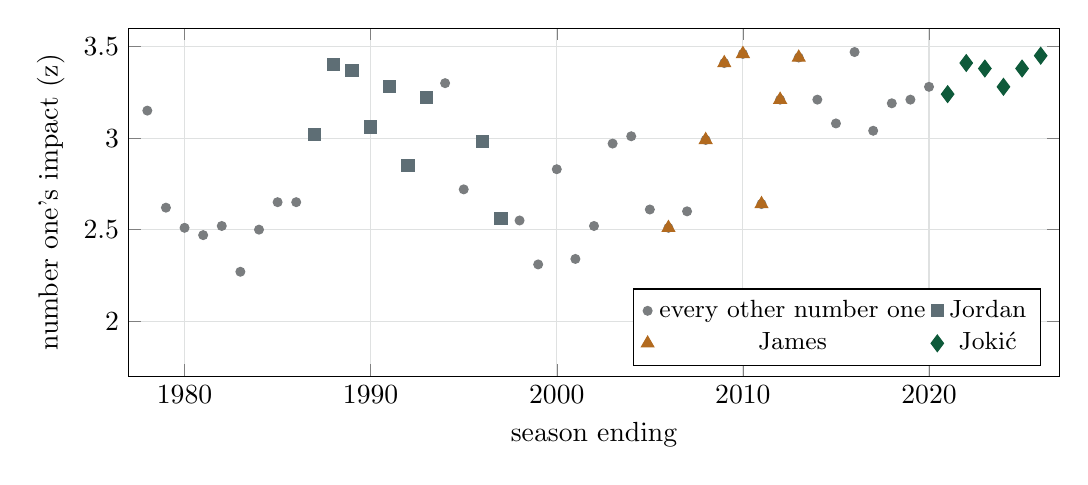
\begin{tikzpicture}
\begin{axis}[
  width=13.4cm, height=6.0cm,
  xmin=1977, xmax=2027, ymin=1.7, ymax=3.6,
  xlabel={season ending}, ylabel={number one's impact (z)},
  xtick={1980,1990,2000,2010,2020}, x tick label style={/pgf/number format/1000 sep=},
  grid=major, grid style={fade!40},
  legend style={font=\small, at={(0.98,0.03)}, anchor=south east, legend columns=2},
]
\addplot[only marks, mark=*, mark size=1.6pt, color=fade!70!black] coordinates {\allfirst};
\addplot[only marks, mark=square*, mark size=2.2pt, color=steel] coordinates {\runJordan};
\addplot[only marks, mark=triangle*, mark size=2.6pt, color=amberx] coordinates {\runLeBron};
\addplot[only marks, mark=diamond*, mark size=3.0pt, color=court] coordinates {\runJokic};
\legend{every other number one, Jordan, James, Jokić}
\end{axis}
\end{tikzpicture}
\caption{The number one's impact per minute, every season since 1977--78. Of the ten highest
single seasons on the chart, four are Jokić's, three are LeBron's, and two are Jordan's. The
highest one is Steph Curry's 2015--16.}
\label{fig:runs}
\end{figure}

Each of these runs tells a different story. Jordan's run was the longest and the most
dominant: he beat the second-best player by 0.61 on average. LeBron's run won the most MVPs,
with four. Jokić's run is statistically ``the best.'' His six seasons have an average impact
score of +3.36, above Jordan's +3.17 and LeBron's +3.19. Jokić's worst season at number one,
+3.24, is higher than the best seasons Larry Bird, Shaq, or Julius Erving ever had. Jordan had
one edge over Jokić: margin. Jokić led by just 0.10 and 0.15 in the last two seasons, with
Shai Gilgeous-Alexander right behind him both times. Being the best in our model and being
the most dominant are two different things, and Jokić can only claim one of them.

\section*{The voters}

The MVP went to our number one in 24 of 49 seasons, and the typical winner ranked second in
our data. In most years the winner stays within our top three, and the voters probably also
weigh team success. However, some of the misses have been huge. Moses Malone won in 1978--79
while 14th in our rankings, and Steve Nash won in 2004--05 while ranked 12th.

Jordan was our number one in nine seasons and only won the MVP in four of those. Magic
Johnson took three of the other five, and Charles Barkley and Karl Malone also took one each.
Jokić has lost three of his six: to Joel Embiid in 2022--23 and to SGA in the last two
seasons.\src{3}{https://www.basketball-reference.com/awards/awards_2026.html} Part of that
is voter fatigue. Once a player has a few MVPs on the shelf, voters start looking for a new
story, and Jokić already has three. By the standards of the last 50 years, that's completely
normal. Our model's best player loses the vote roughly half the time, so if you think Jokić
has been robbed, you're kind of wrong.

\section*{Why The 644 has it closer}

Everything you read above comes from \gravity{} Historical. Our actual ranking, The 644,
gives Jokić a rating of 97.8, 4.9 points ahead of SGA in second at
92.9.\src{5}{https://thegravityreport.com/the644/the644-2026-07.csv} That's a tighter race
than the historical model shows, for two reasons, and only one of them is a flaw. The flaw is
ours: the model limits every input at four standard deviations above average, and Jokić's
2025--26 Box Plus/Minus sat at 4.66. The cap takes about 3 points off his
rating.\src{4}{https://thegravityreport.com/notes/spec/} The other reason is fair. The model
took away 3.4 points because of his playoff BPM (8.0 in a six-game series loss to Minnesota),
which was well below his regular-season 14.2. Playoff performance is a real metric, and it
should count. Cleaning the Glass, which filters out garbage time, shows the playoff dip
clearly: his points per 100 shot attempts fell from 133.5 to 111.5 in the series, and he shot
only 20\% from three.\src{7}{https://cleaningtheglass.com/stats/player/1883}

\section*{The seventh year}

Does a number one usually keep his spot? History gives three different answers, depending on
which number ones you look at. Looking at all of them, our number one has kept that spot the
following season 30 times out of 46. Looking only at the ones whose margin was 0.15 or less,
like Jokić's is right now, the rate drops to 7 out of 11. Looking only at the ones who were 30
or older, it was just 3 out of 7, and Jokić is 31 this season.

The rivals matter more than the base rates do, so let's project each number one candidate from
his 2025--26 season. Table~\ref{tab:scen} lays it out. If Jokić repeats his season, his gravity
score rises to 100.7. If SGA repeats his, he scores 95.4. To reach a score of 100, SGA would
need to improve his impact by 0.4, which is exactly the gap between him and Jokić last season.
In other words, he would have to play like Jokić did. Victor Wembanyama jumped by 1.2 last
season to reach +2.7. Another jump of 0.8 on top of that would get him to 98.6, still short of
a repeating Jokić. The last row is the aging risk. A typical star loses 0.29 of impact between
30 and 31. If that happens to Jokić, his score next year is 97.4, which puts him ahead of an
SGA who repeats and behind an SGA who improves.

\begin{table}[h]
\centering\small
\caption{July 2027 gravity scores under each scenario. Impact here is the full model's
(it includes on/off), so the levels differ slightly from Table~\ref{tab:all}.}
\begin{tabular}{llcc}
\toprule
Scenario & What it assumes & 2026--27 impact & July 2027 score \\
\midrule
Jokić repeats 2025--26 & 65 games, no playoff charge & $+3.43$ & \textbf{100.7} \\
SGA repeats 2025--26 & same season again & $+3.03$ & 95.4 \\
SGA improves by 0.4 & plays like Jokić did, 72 games & $+3.43$ & 100.0 \\
Wembanyama repeats & same season again & $+2.74$ & 89.6 \\
Wembanyama improves by 0.8 & another leap, 72 games & $+3.54$ & 98.6 \\
Jokić ages like a typical star & loses 0.29, 68 games & $+3.13$ & 97.4 \\
\bottomrule
\end{tabular}
\label{tab:scen}
\end{table}

We think Jokić has a 55\% chance of getting his seventh year in a row as the \gravity{}
number one. Our external prediction is that Jokić will have the best BPM in the league, which
ironically he's also done six years in a row. The BPM leader has repeated 34 of 52 times, and
15 of 21 times once the leader had three or more titles in a row. We think this one has about a
60\% chance. The betting market says his MVP chances are 17\%, or +500 on DraftKings. We think
it's really a 25\% chance, considering we think he's more likely than not to be the best
player in the league.\src{6}{https://www.vegasinsider.com/nba/odds/mvp/}

\forecastscale
\forecastitem{55}{Nikola Jokić ranks \#1 in The 644, July 2027 edition.}{\#1 = Win \quad
\#2 = Near miss (graded as a miss) \quad \#3 or below = Miss. This is our own ranking; we keep
one bet on it each article so the model gets graded too.}
\forecastitem{60}{Nikola Jokić leads the NBA in 2026--27 Box Plus/Minus among players with
1,500+ regular-season minutes.}{Basketball Reference, final regular-season table.}
\forecastitem{25}{Nikola Jokić wins the 2026--27 MVP award.}{NBA's official announcement.}

\medskip\noindent{\footnotesize\textcolor{steel}{External predictions are graded by April 30,
2027 (BPM) and June 30, 2027 (MVP). Registered October 17, 2026, before the
October 18 freeze. Scored by Brier score in the Forecast Ledger.}}

\section*{Method and sources}
\small
\gravity{} Historical (\gravity-RS in the code): 0.533 $z_{\mathrm{BPM}}$ + 0.133 $z_{\mathrm{WS/48}}$ + 0.333 $S'$, with the
specification's small-sample shrink, minutes-weighted moments over players with 200+
minutes, clipped at $\pm 4$. Code: \texttt{papers/common/gravity\_rs.py},
\texttt{papers/jokic/history.py}, \texttt{papers/jokic/analysis.py}.
\begin{enumerate}[label={[\arabic*]}]
\item Basketball Reference, league advanced and per-100 tables, 1977--78 to 2025--26. \url{https://www.basketball-reference.com/leagues/}
\item Basketball Reference, NBA MVP winners. \url{https://www.basketball-reference.com/awards/mvp.html}
\item Basketball Reference, 2025--26 awards voting. \url{https://www.basketball-reference.com/awards/awards_2026.html}
\item The Gravity Report, The \gravity{} Specification, v3. \url{https://thegravityreport.com/notes/spec/}
\item The Gravity Report, The 644, July 2026 edition (CSV). \url{https://thegravityreport.com/the644/the644-2026-07.csv}
\item VegasInsider, MVP odds (DraftKings, September 28, 2026). \url{https://www.vegasinsider.com/nba/odds/mvp/}
\item Cleaning the Glass, Nikola Jokić (garbage time filtered), accessed September 29, 2026. \url{https://cleaningtheglass.com/stats/player/1883}
\end{enumerate}

\end{document}
